\documentclass[14pt,aspectratio=1610]{beamer}
%\documentclass[14pt,aspectratio=1610,handout]{beamer}
\usepackage{csu-theme}
\usepackage{arrays}
\usepackage{linked-lists}
\usetikzlibrary{backgrounds}

\usepackage{subcaption}
\usepackage{xparse} %  to have commands with multiple optional parameters
\usepackage{pgf-umlcd}
\usepackage{tikz}
\usetikzlibrary{shapes.multipart, positioning}
\tikzset{
  stack/.style={%
    rectangle split,
    rectangle split parts=#1,
    draw,
    anchor=center,
    minimum width=12mm,
    minimum height=4mm,
    font=\tiny,
    very thick,
    line join=bevel,
    fill=CSUcyan,
    text=black,
  },
  stack top/.style={%
    rectangle, draw, minimum size=12mm - 1pt,
    yslant=0.5,xslant=-1, anchor=south west,
    very thick,
    xshift=-1pt,
    yshift=-1pt,
    line join=bevel,
    fill=CSUcyan,
    text=black,
  },
  stack instruction/.style={anchor=west, align=left, inner sep=0pt}
}
\newcommand{\Stack}[2][stack]{%

  

  % Left of Stack
  \node[stack=#2, yslant=-0.5, anchor=south east, xshift=1pt] (A) {
    #1
    % \foreach \element in {#2} {
    %   \nodepart{name}\element
    % }
  };

  % Right of Stack
  \node[stack=#2, yslant=0.5, anchor=south west, xshift=-1pt] (B) {
      #1
      % \foreach \element in {#1} {
      %   \nodepart{#1}\element
      % }
  };

  
  % Top of Stack
  \node at (A.north east)  [anchor=west, shift={(-1pt, 0.7pt)}, stack top] (StackTop) {
    \rotatebox{-45}{#1}
  };
  
}


%%% Circular Array %%%
\usepackage{xstring}

% https://tex.stackexchange.com/questions/21559/macro-to-access-a-specific-member-of-a-list/21560#21560
\newcommand*\GetListMember[2]{\StrBetween[#2,\number\numexpr#2+1]{,#1,},,\par}%

\newlength{\MidRadius}
\newcommand*{\CircularSequence}[3]{%
    % #1 = outer circle radius
    % #2 = inner circle radius
    % #3 = seqeunce
    \StrCount{#3}{,}[\NumberOfElements]
    \pgfmathsetmacro{\AngleSep}{360/(\NumberOfElements+1)}
    \pgfmathsetlength{\MidRadius}{(#1+#2)/2}
    \fill[CSUcyan,even odd rule] (0,0) circle (#1) (0,0) circle (#2);
    \draw [very thick] circle (#2);
    \draw [very thick] circle (#1);
    \foreach [count = \Count] \Angle in {0,\AngleSep,..., 360} {%
        \draw [very thick] (\Angle:#2) -- (\Angle:#1);
        \pgfmathsetmacro{\MidPoint}{\Angle+\AngleSep/2}
        \node [text=black] at (\MidPoint:\MidRadius) {\GetListMember{#3}{\Count}};
    }%
}%

%%% End Circular Array %%%

\setlength{\parskip}{0.5em}

\title{\Huge{} Stacks and Queues}
\subtitle{CSCI 315: Data Structure Analysis\\Chapter 17}
%\author{Sean T. Hayes, Ph.D.}
\institute{Charleston Southern University}

%% Comment out date to use default (today)
% \date{February 20, 2025}
\subject{Software Programming}
%\keywords{}
\graphicspath{{../imgs/stack-queue}}

\begin{document}

\begin{frame}
  \titlepage{}
\end{frame}

\section{Introduction}

\begin{frame}{Objectives: Stacks}
In this lecture, you will:
\begin{itemize}
\item
  Learn about stacks.
\item
  Examine various stack operations.
\item
  Learn how to implement a stack as an array.
\item
  Learn how to implement a stack as a linked list.
\item
  Learn how to use a stack to solve problems like removing recursion.
\end{itemize}
\end{frame}

\begin{frame}{Objectives: Queues}
In this lecture, you will:
\begin{itemize}
\item
  Learn about queues.
\item
  Examine various queue operations.
\item
  Learn how to implement a queue as an array.
\item
  Learn how to implement a queue as a linked list.
\item
  Discover how to use queues to solve simulation problems.
\end{itemize}
\end{frame}

\begin{frame}{Stacks}
Stack: a data structure in which elements are added and removed from one end only.

\begin{itemize}
\item
  Addition and deletion occurs only at the top of the stack.
\item
  Last in, first out (LIFO) data structure
\item
  Operations:
  \begin{itemize}
  \item
    Push: to add an element onto the stack
  \item
    Pop: to remove an element from the stack
  \end{itemize}
\end{itemize}
\end{frame}

\begin{frame}{Various types of stacks}

\begin{figure}
\centering
\begin{subfigure}{0.2\textwidth}
  
\includegraphics[width=\textwidth]{stack-example-coins}
  \caption{Stack of Coins}%
\label{fig:coins}
\end{subfigure}
\hfill
\begin{subfigure}{0.2\textwidth}
  
\includegraphics[width=\textwidth]{stack-example-trays}
  \caption{Stack of Trays}%
  \label{fig:trays}
\end{subfigure}
\hfill
\begin{subfigure}{0.22\textwidth}
  \centering
  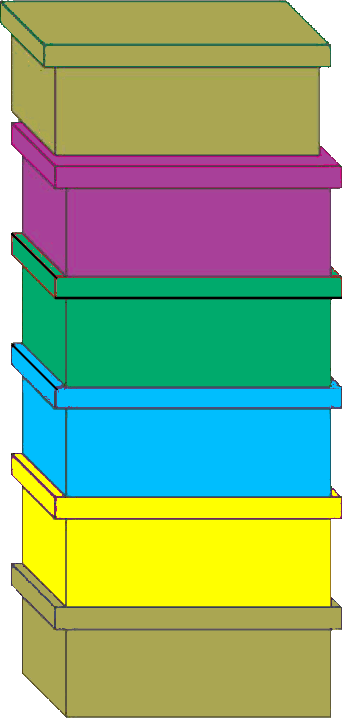
\includegraphics[width=0.75\textwidth]{stack-example-boxes}
  \caption{Stack of Boxes}%
  \label{fig:boxes}
\end{subfigure}
\hfill
\begin{subfigure}{0.3\textwidth}
  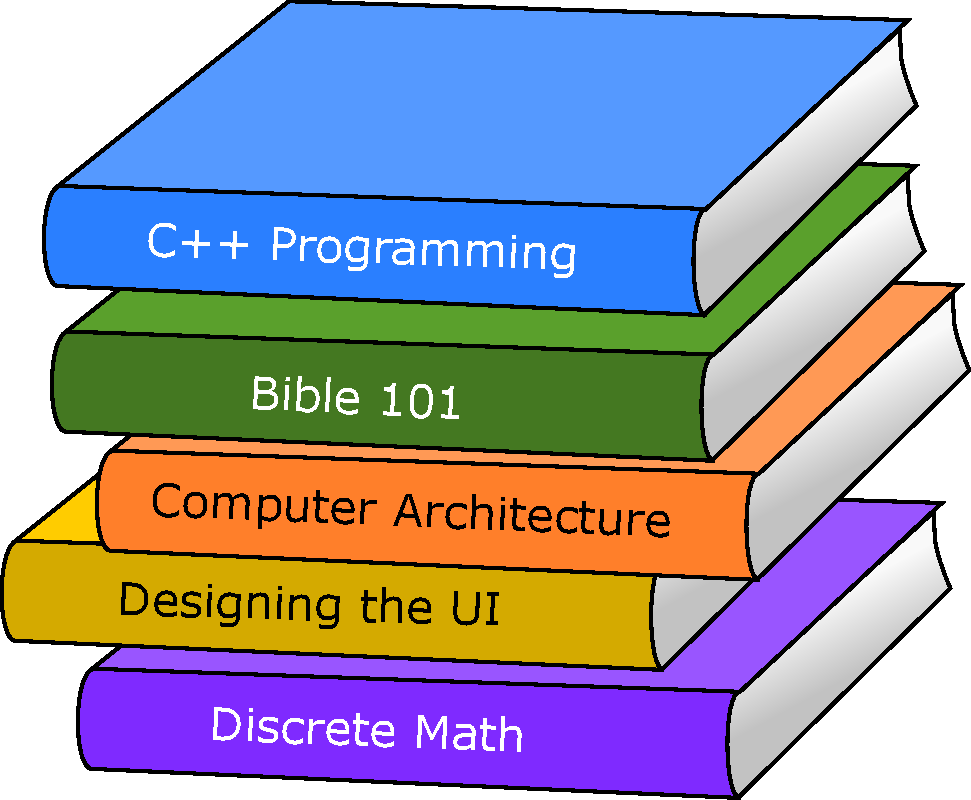
\includegraphics[width=\textwidth]{stack-example-books}
  \caption{Stack of Books}%
  \label{fig:books}
\end{subfigure}
%
% \caption{Creating subfigures in \LaTeX.}
\label{fig:figures}
\end{figure}
\end{frame}

\begin{frame}{Stack Example}
\begin{columns}[b]
  \column{0.66\textwidth}
    \onslide<1>{\begin{tikzpicture}
      \Stack[A]{1}
    \end{tikzpicture}}\hspace{5mm}
    \onslide<-2>{\begin{tikzpicture}
      \Stack[B]{1}
    \end{tikzpicture}}

    \onslide<-3>{\hspace{1cm}\begin{tikzpicture}
      \Stack[C]{1}
    \end{tikzpicture}}\hspace{5mm}
    \onslide<-5>{\begin{tikzpicture}
      \Stack[D]{1}
    \end{tikzpicture}}

    \onslide<-6>{\begin{tikzpicture}
      \Stack[E]{1}
    \end{tikzpicture}}

  \column{0.33\textwidth}
    \centering
    \begin{tikzpicture}
      \only<1>{
        \node (stack) at (0,0)  [stack top, font=\tiny, align=center, name=stack]{};
        \node at (stack) [anchor=center, name=stack, align=left, yslant=0.5, xslant=-1, font=\footnotesize, text=black]{Empty\\Stack};
      }
      \only<2>{
        \Stack[A]{1}
        \node[above = of StackTop, align=center, anchor=center] {Push\\A};
      }
      \only<3>{
        \Stack[B]{2}
        \node[above = of StackTop, align=center, anchor=center] {Push\\B};
      }
      \only<4>{
        \Stack[C]{3}
        \node[above = of StackTop, align=center, anchor=center] {Push\\C};
      }
      \only<5>{
        \Stack[C]{3}
        \node[above = of StackTop, align=center, anchor=center] {Peek\\top};
      }
      \only<6>{
        \Stack[D]{4}
        \node[above = of StackTop, align=center, anchor=center] {Push\\D};
      }
      \only<7>{
        \Stack[E]{5}
        \node[above = of StackTop, align=center, anchor=center] {Push\\E};
      }
      \only<8>{
        \Stack[D]{4}
        \node[above = of StackTop, align=center, anchor=center] {Pop};
      }
      \only<9>{
        \Stack[C]{3}
        \node[above = of StackTop, align=center, anchor=center] {Pop};
      }
      
      % Reserve the space for the biggest stack size
      \invisible{\Stack{5}\node[above = of StackTop, align=center, anchor=center] {Push\\E};}
    \end{tikzpicture}
\end{columns}

\end{frame}

\begin{frame}{Stack Interface}
  \renewcommand{\umlfillcolor}{CSUblue!80!black}
  \renewcommand{\umldrawcolor}{white}
  \renewcommand{\umltextcolor}{white}
  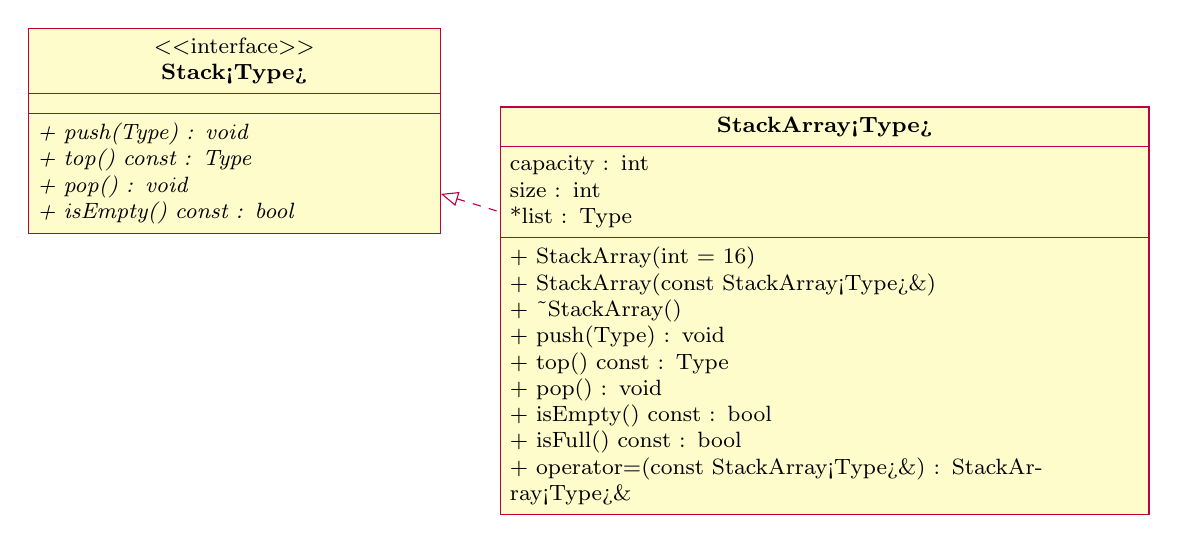
\begin{tikzpicture}[every node/.style={font=\footnotesize}]
    \begin{interface}{Stack<Type>}{0,0}
      \operation[0]{+ push(Type) : void}
      \operation[0]{+ top() const : Type}
      \operation[0]{+ pop() : void}
      \operation[0]{+ isEmpty() const : bool}
    \end{interface}

    \begin{class}[text width=8cm]{StackArray<Type>}{7.5,-1}
      \implement{Stack<Type>}
      \attribute{capacity : int}
      \attribute{size : int}
      \attribute{*list : Type}
      \operation{+ StackArray(int = 16)}
      \operation{+ StackArray(const StackArray<Type>\&)}
      \operation{+ \textasciitilde{}StackArray()}
      \operation{+ push(Type) : void}
      \operation{+ top() const : Type}
      \operation{+ pop() : void}
      \operation{+ isEmpty() const : bool}
      \operation{+ isFull() const : bool}
      \operation{+ operator=(const StackArray<Type>\&) : StackArray<Type>\&}
    \end{class}
  \end{tikzpicture}
\end{frame}

\section{Array Stack}
% \begin{frame}{Stack Operations}
% In the abstract Stack class, we may want the following operations
% \begin{itemize}
% \item
%   \lstinline{StackArray(const int capacity = 8)}
% \item
%   \lstinline{StackArray(const StackArray<Type>& src)}
% \item
%   \lstinline{isEmpty() const}
% \item
%   \lstinline{isFull() const}
% \item
%   \lstinline{push()}
% \item
%   \lstinline{top() const}
% \item
%   \lstinline{pop()}
% \item
%   ...
% \end{itemize}

% \end{frame}

\begin{frame}{Array-Based Stack Implementation}
\begin{itemize}
\item
  The first element goes in the first array position, the second in the second position, etc.
\item
  The top of the stack is an index of the last element added to the stack.
\item
  Stack elements may be stored in an array, which is a random-access data structure.
  \begin{itemize}
  \item
    The stack element is accessed only through the top.
  \end{itemize}
\item
  To track the top position, use a variable.
\end{itemize}

\end{frame}


\begin{frame}{Array-Based Stack Implementation}
\begin{itemize}
\item
  Can dynamically allocate an array.
\item
  Enables the user to specify the size of the array.
\end{itemize}
\end{frame}

\begin{frame}{Array-Based Stack Implementation}
\begin{itemize}
\item
  The \texttt{size} attribute will hold the number of elements currently in the array.
\item
  Therefore, we will use \texttt{size - 1} as the top of the stack.
\item
  The \texttt{capacity} attribute will hold the maximum number of elements of the array before it needs to be resized.
\end{itemize}
\end{frame}

\begin{frame}{Array-Based Stack Implementation}
  \begin{tikzpicture}

    % Dynamic Array
    \ArrayLabel{}
    \ArrayNodeStack{A}
    \ArrayNodeStack{B}
    \ArrayNodeStack{C}
    \ArrayNodeStack{D}
    \onslide<2->{\ArrayGroupVerticleRight{elD}{elA}{Stack Elements}}
    \ArrayNodeStackSpan{}
    \ArrayNodeStack[CSUcyan][{[99]}]{}
    \onslide<3->{\ArrayGroupVerticleRight{prev}{space}{Unused}}

    % Stack Class Members
    \begin{scope}[node of array/.append style={minimum width=14mm}]
      \ArrayLabel[0][-3]{}
      \ArrayNodeStack[CSUgold][pList]{}
      \fill (prev) circle(3pt);
      \coordinate (ptrCircle) at (prev);
      \draw[link] (ptrCircle) to[bend right] (elA);

      \ArrayNodeStack[CSUcyan][size]{4}
      \ArrayNodeStack[CSUcyan][capacity]{100}
    \end{scope}
    \begin{scope}[on background layer]
      \node[draw,fill=CSUslate, very thick,fit=(el100) (el4) (el) (index)] (stackMembers) {};
    \end{scope}
    \node[anchor=south, font=\ttfamily] at ([yshift=0pt] stackMembers.north) {stack};
  \end{tikzpicture}
\end{frame}

\begin{frame}{Empty Array-Based Stack}
  \begin{tikzpicture}

    % Dynamic Array
    \ArrayLabel{}
    \ArrayNodeStack{A}
    \ArrayNodeStack{B}
    \ArrayNodeStack{C}
    \ArrayNodeStack{D}
    %\ArrayGroupVerticleRight{elD}{elA}{Stack Elements}
    \ArrayNodeStackSpan{}
    \ArrayNodeStack[CSUcyan][{[99]}]{}
    \ArrayGroupVerticleRight{prev}{elA}{Unused}

    % Stack Class Members
    \begin{scope}[node of array/.append style={minimum width=14mm}]
      \ArrayLabel[0][-3]{}
      \ArrayNodeStack[CSUgold][pList]{}
      \fill (prev) circle(3pt);
      \coordinate (ptrCircle) at (prev);
      \draw[link] (ptrCircle) to[bend right] (elA);

      \ArrayNodeStack[CSUcyan][size]{0}
      \ArrayNodeStack[CSUcyan][capacity]{100}
    \end{scope}
    \begin{scope}[on background layer]
      \node[draw,fill=CSUslate, very thick,fit=(el100) (el4) (el) (index)] (stackMembers) {};
    \end{scope}
    \node[anchor=south, font=\ttfamily] at ([yshift=0pt] stackMembers.north) {stack};
  \end{tikzpicture}
\end{frame}

\begin{frame}{Empty Array-Based Stack}
  \begin{tikzpicture}[stack instruction/.append style={fit={(stackMembers.east) (stackMembers.west)}, yshift=5em}]

    % Dynamic Array
    \ArrayLabel{}
    \alt<1>{
      \ArrayNodeStack{A}
    }{
      \ArrayNodeStack{u}
    }
    \alt<-3>{
      \ArrayNodeStack{B}
    }{
      \ArrayNodeStack{s}
    }
    \alt<-5>{
      \ArrayNodeStack{C}
    }{
      \ArrayNodeStack{c}
    }
    \ArrayNodeStack{D}
    %\ArrayGroupVerticleRight{elD}{elA}{Stack Elements}
    \ArrayNodeStackSpan{}
    \ArrayNodeStack[CSUcyan][{[99]}]{}

    \alt<1>{
      \ArrayGroupVerticleRight{prev}{elA}{Unused}
    }{
      \alt<-3>{
        \ArrayGroupVerticleRight{prev}{elB}{Unused}
      }{
        \alt<-5>{
          \ArrayGroupVerticleRight{prev}{elC}{Unused}
        }{
          \alt<-8>{
            \ArrayGroupVerticleRight{prev}{elD}{Unused}
          }{
            \ArrayGroupVerticleRight{prev}{elc}{Unused}
          }

        }
      }
    }

    \alt<1>{
    }{
      \alt<-3>{
        \ArrayGroupVerticleRight{elu}{elu}{Stack Elements}
      }{
        \alt<-5>{
          \ArrayGroupVerticleRight{els}{elu}{Stack Elements}
        }{
          \alt<-8>{
            \ArrayGroupVerticleRight{elc}{elu}{Stack Elements}
          }{
            \ArrayGroupVerticleRight{els}{elu}{Stack Elements}
          }

        }
      }
    }


    % Stack Class Members
    \begin{scope}[node of array/.append style={minimum width=14mm}]
      \ArrayLabel[0][-3]{}
      \ArrayNodeStack[CSUgold][pList]{}
      \fill (prev) circle(3pt);
      \coordinate (ptrCircle) at (prev);
      \draw[link] (ptrCircle) to[bend right] (elA);

      \alt<1>{
        \ArrayNodeStack[CSUcyan][size]{0}
      }{
        \alt<-3>{
          \ArrayNodeStack[CSUcyan][size]{1}
        }{
          \alt<-5>{
            \ArrayNodeStack[CSUcyan][size]{2}
          }{
            \alt<-8>{
              \ArrayNodeStack[CSUcyan][size]{3}
            }{
              \ArrayNodeStack[CSUcyan][size]{2}
            }
          }
        }
      }
      \ArrayNodeStack[CSUcyan][capacity]{100}
    \end{scope}
    \begin{scope}[on background layer]
      \node[draw,fill=CSUslate, very thick,fit=(el100) (el4) (el) (index)] (stackMembers) {};
    \end{scope}
    \node[anchor=south, font=\ttfamily] at ([yshift=0pt] stackMembers.north) {stack};

    % Task
    \alt<-2>{
      \node[stack instruction] at (stackMembers.north) {Push \lstinline{'u'}.};
    }{
      \alt<-4>{
        \node[stack instruction] at (stackMembers.north) {Push \lstinline{'s'}.};
      }{
        \alt<-6>{
          \node[stack instruction] at (stackMembers.north) {Push \lstinline{'c'}.};
        }{
          \alt<-7>{
            \node[stack instruction] at (stackMembers.north) {The top is \lstinline{'c'}.};
          }{
            \alt<-9>{
              \node[stack instruction] at (stackMembers.north) {Pop.};
            }{
              \node[stack instruction] at (stackMembers.north) {The top is \lstinline{'s'}.};
            }
          }
        }

      }
    }
    \onslide<10>{}
  \end{tikzpicture}
\end{frame}


\section{Linked Stack}


\begin{frame}{Linked Implementation of a Stack}
\begin{itemize}[<+->]
\item
  Array only allows a fixed number of elements.
\item
  If the number of elements to be pushed exceeds the array size, the program may terminate.
\item
  Linked lists can dynamically organize data.
\item
  In a linked representation, \texttt{mpHead} is a pointer to the memory address of the top element in the stack.\\
  (\texttt{mpHead} may be named \texttt{mpStackTop})
\end{itemize}
\end{frame}


\begin{frame}{Linked-List Implementation of a Stack}
  \begin{tikzpicture}[stack instruction/.append style={yshift=3em, anchor=north west}]

  \LinkPtr{mpStackTop}
  \only<7->{
    \LinkedNode{C}
  }
  \only<5->{
    \LinkedNode{B}
  }
  \onslide<3->{
    \LinkedNode{A}
  }

  \only<1>{
    \node[stack instruction] at (head.west) {Empty stack.};
  }
  
  \onslide<2->{
    \alt<-3>{
      \node[stack instruction] at (head.west) {Push \lstinline{'A'}.};
    }{
      \alt<-5>{
        \node[stack instruction] at (head.west) {Push \lstinline{'B'}.};
      }{
        \node[stack instruction] at (head.west) {Push \lstinline{'C'}.};
      }
    }
  }

  % Reserve space for this on a future slide
  \invisible{\LinkPtr[-2]{pNewNode}\LinkedNode{D}}
  \onslide<7>{}
  \end{tikzpicture}
\end{frame}

\begin{frame}{Push}
  \begin{tikzpicture}[stack instruction/.append style={yshift=3em, anchor=north west}]

  \LinkPtr{mpStackTop}
  \coordinate (mpStackTop) at (ptr);
  \alt<-3>{
    \LinkedNode{C}
  }{
    \LinkedNode[ptr][false]{C}
  }

  \LinkedNode{B}
  \LinkedNode{A}

  \node[stack instruction] at (head.west) {Push \lstinline{'D'}.};

  \onslide<2->{
    \LinkPtr[-2]{pNewNode}
    \LinkedNode{D}
    \onslide<4->{
      \draw[link] (mpStackTop) to [bend right=10] (elD);
    }
    \onslide<3->{
      \draw[link] (ptr) to [bend right=10] (elC);
    }
  }
  \end{tikzpicture}
\end{frame}

\begin{frame}{Pop}
  \begin{tikzpicture}[stack instruction/.append style={yshift=3em, anchor=north west}]

  \LinkPtr{mpStackTop}
  \coordinate (mpStackTop) at (ptr);
  \alt<-2>{
    \LinkedNode{D}
  }{
    \onslide<-3>{
      \LinkedNode[ptr][false]{D}
    }
  }
  \onslide<2->{
    \alt<-3>{
      \TailPtr{pToDelete}
    }{
      \TailPtr[null]{pToDelete}
    }
  }
  \alt<-3>{
    \LinkedNode{C}
  }{
    \LinkedNode[ptr][false]{C}
  }
  \LinkedNode{B}
  \LinkedNode{A}

  \onslide<3->{\draw[link] (mpStackTop) to [bend left] (elC);}

  \node[stack instruction] at (head.west) {Pop.};
  \onslide<4>{}

  % Reserve space for this on a future slide
  \invisible{\LinkPtr[-2]{pNewNode}\LinkedNode{D}}
  \end{tikzpicture}
\end{frame}

\section{Postfix Notation}

\begin{frame}{Infix Notation}
\emph{Infix notation}: usual notation for writing arithmetic expressions
\begin{itemize}[<+->]
\item
  Operator is written between the operands.
\item
  Example: $a + b$.
\item
  Evaluates from left to right.
\item
  Operators have precedence.
\item
  Parentheses can be used to override precedence.
\end{itemize}
\end{frame}

\begin{frame}{Prefix Notation (Polish Notation)}
\emph{Prefix (Polish) notation}: operators are written before the operands
\begin{itemize}
\item
  Introduced by the Polish mathematician Jan Lukasiewicz in the early 1920s.
\item
  Parentheses can be omitted.
\item
  Example: $a + b$ becomes $+\ a\ b$.
\end{itemize}
\end{frame}

\begin{frame}{Postfix Notation (Reverse Polish Notation)}
\emph{Postfix notation}: operators follow the operands (postfix operators)

\begin{itemize}
\item
  Proposed by Australian philosopher and early computer scientist, Charles L. Hamblin, in the late 1950s.
\item
  Advantage: operators appear in the order required for computation.
\item
  Example: $a + b \cdot c$ becomes $a\ b\ c\ \cdot\ +$
\item
  Example: $(a + b) \cdot c$ becomes $a\ b + c\ \cdot$
\end{itemize}
\end{frame}

\begin{frame}{Postfix Notation Examples}
\center{%
\begin{tabular}{l l}
\hline
  \textbf{Infix Expression} & \textbf{Equivalent Postfix Express}\\
\hline
  $a + b$ & $a\ b\ +$\\
  $a + b \cdot c$ & $a\ b\ c \cdot +$\\
  $a \cdot b + c$ & $a\ b \cdot c\ +$\\
  $(a + b) \cdot c$ & $a\ b + c\ \cdot$\\
  $(a - b) \cdot (c + d)$ & $a\ b - c\ d\ +\ \cdot$\\
  $(a + b) \cdot (c - d / e)$ & $a\ b + c\ d\ e\ /\ -\ \cdot$\\
  $(a + b) \cdot (c - d / e) + f$ & $a\ b + c\ d\ e\ /\ -\ \cdot\ f\ +$\\
\hline
\end{tabular}}
\end{frame}

\begin{frame}{Postfix Expressions Calculator}
Postfix notation has important applications in computer science.

Many compilers first translate arithmetic expressions into postfix notation and then translate this expression into machine code.

Evaluation algorithm:\vspace{-0.5em}
\begin{itemize}
  \item
    Scan expression from left to right.
  \item
    When an operator is found, back up to get operands, perform the operation, and continue.
\end{itemize}
\end{frame}

\begin{frame}{Postfix Expressions Calculator}
Expression: $6\ 3 + 2\ *\ =$


\begin{columns}
\column{0.6\textwidth}
  \alt<-2>{%
    Push \lstinline{6} onto the stack.
  }{%
    \alt<-4>{%
      Push \lstinline{3} onto the stack.
    }{%
      \alt<-7>{%
        \lstinline{+}\\
        Pop stack twice.\\
        op2 = 3;\\
        op1 = 6;
      }{%
        \alt<-9>{
          \lstinline{op1 + op2 = 9}\\
          Push \lstinline{9} onto the stack.
        }{
          \alt<-11>{
            Push \lstinline{2} onto the stack.
          }{
            \alt<-16>{
              \lstinline{*}\\
              Pop stack twice.\\
              op2 = 2;\\
              op1 = 9;
            }{
              \alt<-18>{
                \lstinline{op1 * op2 = 18}\\
                Push \lstinline{18} onto the stack.
              }{
                \lstinline{=}\\
                Pop stack and print: \lstinline{18}\\
              }

            }

          }
        }
      }
    }
  }

\column{0.3\textwidth}
  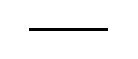
\begin{tikzpicture}[span of array/.append style={minimum height=8mm,}, stack instruction/.append style={anchor=south}]
    % Line representing the empty stack.
    \draw[very thick] (-5mm, 0.36) to (5mm, 0.36);
    \ArrayLabel{Stack}
    \alt<-7>{
      \onslide<2-6>{
        \ArrayNodeStackSpan[6]{}
      }

      \onslide<4-5>{
        \ArrayNodeStackSpan[3]{}
      }
    }{
      \alt<-17>{
        \onslide<9-13>{\ArrayNodeStackSpan[9]{}}
        \onslide<11-12>{\ArrayNodeStackSpan[2]{}}
      }{
        \onslide<18-19>{\ArrayNodeStackSpan[18]{}}
        \onslide<1>{\ArrayNodeStackSpan[]{}} % Never displayed but holds space.
      }
    }

  \onslide<20>{}
  \end{tikzpicture}
\end{columns}
\end{frame}

\begin{frame}{Postfix Expressions Calculator}
Symbols can be numbers or anything else:
\begin{itemize}
  \item
    $+$, $-$, $*$, and $/$ are operators, require two operands.
  \begin{itemize}
    \item
      Pop stack twice and evaluate the expression.
    \item
      If the stack has less than two elements, then error.
  \end{itemize}
  \item
    If the symbol is $=$, the expression ends.
    \begin{itemize}
      \item
        Pop and print the answer from the stack.
      \item
        If the stack has more than one element, then error.
    \end{itemize}
  \item
    If the symbol is anything undefined, the expression contains an illegal operator.
\end{itemize}
\end{frame}

\begin{frame}[fragile]{Postfix Expressions Calculator}
Start to the function:
\begin{lstlisting}
bool evaluatePostfixExpression(ifstream &input, double& result)
{
  Stack<double> stack;
  char nextSymbol;
  double value;

  // ...
  nextSymbol = input.peek();
  // ...
}
\end{lstlisting}
\end{frame}


% \begin{frame}{Postfix Expressions Calculator}
% Assume postfix expressions are in this form:\\
% \texttt{\#6 \#3 + \#2 * =}
% \begin{itemize}
%   \item
%     If symbol scanned is \#, next input is a number
%   \item
%     If the symbol scanned is not \#, then it is:
%     \begin{itemize}
%       \item
%         An operator (may be illegal) or
%       \item
%         An equal sign (end of expression)
%     \end{itemize}
%   \item
%     Assume the expressions contain only $+$, $-$, $*$, and $/$ operators.
% \end{itemize}
% \end{frame}

% \begin{frame}[fragile]{Postfix Expressions Calculator}
% Pseudocode:\\
% \begin{lstlisting}
% Read the first character
% while not the end of the input data
% {
%   a. initialize the stack
%   b. process the expression
%   c. output the result
%   g. get the next expressions
% }
% \end{lstlisting}
% \end{frame}

\section{SLList in Reverse}

\begin{frame}{Iterating Over a Linked List in Reverse}
\begin{itemize}
  \item
    To print a list backward non-recursively, first get to the last node of the list.
    \begin{itemize}
      \item
        Problem: Links go in only one direction.
      \item
        Solution: Save a pointer to each node in a stack.\\
        Uses the LIFO principle.
    \end{itemize}
  \item
    Since the number of nodes is usually not known, use the linked implementation of a stack.
\end{itemize}  
\end{frame}

\begin{frame}{Iterating Over a Linked List in Reverse}
  \centering
  \onslide<-8>{
    While \lstinline{pCurrent} is not null, push it on the stack and go to next.
  }
  \onslide<9->{
    While the stack is not empty, access the top and pop.
  }

  \begin{tikzpicture}[span of array/.append style={minimum height=6mm, minimum width=6mm}, stack instruction/.append style={anchor=south}, node of array/.append style = {fill=CSUgold}]
    \LinkPtr{pHead}
    \LinkedNode{5}
    \onslide<2-3>{\TailPtr{pCurrent}}
    \onslide<14-15>{\TailPtr{pCurrent}}
    \LinkedNode{10}
    \onslide<4-5>{\TailPtr{pCurrent}}
    \onslide<12-13>{\TailPtr{pCurrent}}
    \LinkedNode{15}
    \onslide<6-11>{
      \alt<8-9>{
        \TailPtr[null]{pCurrent}
      }{
        \TailPtr{pCurrent}
      }
    }

    % Line representing the empty stack.
    \draw[very thick] (-4cm - 3mm, -0.64) to (-4cm + 3mm, -0.64);
    
    \ArrayLabel[-1][-4]{Stack}
    \onslide<3-14>{
      \ArrayNodeStackSpan[]{}
      %\node[pointer, name=ptr2] at (prev) {};
      \fill (prev) circle(2pt);
      \coordinate (ptr) at (prev);
      \draw[link, ->] (ptr) to[bend left] (el5);
    }
    \onslide<5-12>{
      \ArrayNodeStackSpan[]{}
      %\node[pointer, name=ptr2] at (prev) {};
      \fill (prev) circle(2pt);
      \coordinate (ptr) at (prev);
      \draw[link, ->] (ptr) to[bend left] (el10);
    }
    \onslide<7-10>{
      \ArrayNodeStackSpan[]{}
      %\node[pointer, name=ptr2] at (prev) {};
      \fill (prev) circle(2pt);
      \coordinate (ptr) at (prev);
      \draw[link, ->] (ptr) to[bend left] (el15);
    }
    \onslide<15>{}
  \end{tikzpicture}
\end{frame}


\section{Queues}

\begin{frame}{Queues}
  \emph{Queue}: a data structure in which elements are\\
  added from one end (the \textit{back}) and\\
  removed from the other end (the \textit{front}).

  \begin{itemize}
    \item
      First In, First Out (FIFO) data structure
    \item
      Operations: enqueue, dequeue, front, initialize, destroy, check for empty/full queue
    \item
      Can be implemented as an array or linked list.
    \item
      Middle elements should not be accessed directly.
    \item
      Example: Waiting in line in a bank.
  \end{itemize}
\end{frame}

\begin{frame}{Queues Interface}
  \renewcommand{\umlfillcolor}{CSUblue!80!black}
  \renewcommand{\umldrawcolor}{white}
  \renewcommand{\umltextcolor}{white}
  \begin{tikzpicture}[every node/.style={font=\footnotesize}]
    \begin{interface}{Queue<Type>}{0,0}
      \operation[0]{+ push(Type) : void}
      \operation[0]{+ first() const : Type}
      \operation[0]{+ pop() : void}
      \operation[0]{+ isEmpty() const : bool}
      \operation[0]{+ getLength() const : int}
    \end{interface}

    \begin{class}[text width=8cm]{QueueArray<Type>}{7.5,0}
      \implement{Stack<Type>}
      \attribute{capacity : int}
      \attribute{frontIndex : int}
      \attribute{rearIndex : int}
      \attribute{*list : Type}
      \operation{+ QueueArray(int = 16)}
      \operation{+ QueueArray(const QueueArray<Type>\&)}
      \operation{+ \textasciitilde{}QueueArray()}
      \operation{+ push(Type) : void}
      \operation{+ first() const : Type}
      \operation{+ pop() : void}
      \operation{+ isEmpty() const : bool}
      \operation{+ isFull() const : bool}
      \operation[0]{+ getLength() const : int}
      \operation{+ operator=(const QueueArray<Type>\&) : QueueArray<Type>\&}
    \end{class}
  \end{tikzpicture}
\end{frame}

\section{Array Queue}

\begin{frame}{Array-Based Queue Implementation}
  Need \textit{at least} four (member) variables:
  \begin{enumerate}
    \item
      Array to store queue elements
    \item
      \texttt{frontIndex} to track the first element.
    \item
      \texttt{rearIndex} to track the last element
    \item
      \texttt{capacity} to specify the maximum size of the queue.
  \end{enumerate}
\end{frame}

\begin{frame}[fragile,b]{Enqueue Array-Based Implementation}
  To add an element to the queue:

\begin{lstlisting}[basicstyle=\footnotesize\ttfamily]
++mRearIndex; // (Incomplete!) Advance to the next position.
mpList[mIndexRear] = value; // Add element to position
\end{lstlisting}

Example: Enqueue the values A, B, and C.

\begin{tikzpicture}[stack instruction/.append style={fit={(queueMembers.east) (queueMembers.west)}, yshift=5em}]
  % Dynamic Array
  \ArrayLabel[1.5][0]{}
  \ArrayNode{A}
  \node[block] (arrayFirst) [fit=(val)]{};
  \alt<-2>{
    \ArrayNode{}
  }{
    \ArrayNode{B}
  }
  \alt<-4>{
    \ArrayNode{}
  }{
    \ArrayNode{C}
  }
  \ArrayNode{}
  \ArrayNodeSpan{5}
  \ArrayNode{}

    % Queue Class Members
    \begin{scope}[node of array/.append style={minimum width=14mm}]
      \ArrayLabel[0][-2]{}
      \ArrayNodeStack[CSUgold][mpList]{}
      \fill (prev) circle(3pt);
      \coordinate (ptrCircle) at (prev);
      \draw[link] (ptrCircle) to[bend left=10] (arrayFirst);

      \alt<1>{
        \ArrayNodeStack[CSUcyan][mRearIndex]{0}
      }{
        \alt<-3>{
          \ArrayNodeStack[CSUcyan][mRearIndex]{1}
        }{
          \ArrayNodeStack[CSUcyan][mRearIndex]{2}
        }
      }
      \ArrayNodeStack[CSUcyan][mFrontIndex]{0}
      \ArrayNodeStack[CSUcyan][mCapacity]{10}
    \end{scope}
    \begin{scope}[on background layer]
      \node[draw,fill=CSUslate, very thick,fit=(pList) (mFrontIndex) (mRearIndex) (mCapacity)] (queueMembers) {};
    \end{scope}
    \node[anchor=south, font=\ttfamily] at ([yshift=0pt] queueMembers.north) {queue};

    \onslide<5>{}
\end{tikzpicture}
\end{frame}




\begin{frame}[fragile, b]{Dequeue in Array-Based Implementation}
  To remove an element to the queue:

\begin{lstlisting}[basicstyle=\footnotesize\ttfamily]
++mFrontIndex; // (Incomplete!) Advance to the next position.
\end{lstlisting}

Example: Dequeue one value.

\begin{tikzpicture}[stack instruction/.append style={fit={(queueMembers.east) (queueMembers.west)}, yshift=5em}]
  % Dynamic Array
  \ArrayLabel[1.5][0]{}
  \ArrayNode{A}
  \node[block] (arrayFirst) [fit=(val)]{};
  \ArrayNode{B}
  \ArrayNode{C}
  \ArrayNode{}
  \ArrayNodeSpan{5}
  \ArrayNode{}

    % Queue Class Members
    \begin{scope}[node of array/.append style={minimum width=14mm}]
      \ArrayLabel[0][-2]{}
      \ArrayNodeStack[CSUgold][mpList]{}
      \fill (prev) circle(3pt);
      \coordinate (ptrCircle) at (prev);
      \draw[link] (ptrCircle) to[bend left=10] (arrayFirst);
      
      \ArrayNodeStack[CSUcyan][mRearIndex]{2}

      \alt<1>{
        \ArrayNodeStack[CSUcyan][mFrontIndex]{0}
      }{
        \ArrayNodeStack[CSUcyan][mFrontIndex]{1}
      }

      \ArrayNodeStack[CSUcyan][mCapacity]{10}
    \end{scope}
    \begin{scope}[on background layer]
      \node[draw, fill=CSUslate, very thick, fit=(pList) (mFrontIndex) (mRearIndex) (mCapacity)] (queueMembers) {};
    \end{scope}
    \node[anchor=south, font=\ttfamily] at ([yshift=0pt] queueMembers.north) {queue};

    \onslide<2>{}
\end{tikzpicture}
\end{frame}

\begin{frame}[b]{Problem: Unusable Space}
  As we add and remove elements, \lstinline{mRearIndex} and \lstinline{mFrontIndex} only increase, leaving unusable space at the beginning of the array.

  Example state after a sequence of 10 enqueues and 8 dequeues.

\begin{tikzpicture}[stack instruction/.append style={fit={(queueMembers.east) (queueMembers.west)}, yshift=5em}, horizontal span of array/.append style={fill=MyPurple}]
  % Dynamic Array
  \ArrayLabel[1.5][0]{}
  \ArrayNode[MyPurple]{}
  \node[block] (arrayFirst) [fit=(val)]{};
  \ArrayNode[MyPurple]{}
  \ArrayNodeSpan{5}
  \ArrayNode[MyPurple]{}
  \ArrayNode{X}
  \ArrayNode{Y}

  % Queue Class Members
  \begin{scope}[node of array/.append style={minimum width=14mm}]
    \ArrayLabel[0][-2]{}
    \ArrayNodeStack[CSUgold][mpList]{}
    \fill (prev) circle(3pt);
    \coordinate (ptrCircle) at (prev);
    \draw[link] (ptrCircle) to[bend left=10] (arrayFirst);
    \ArrayNodeStack[CSUcyan][mRearIndex]{9}
    \ArrayNodeStack[CSUcyan][mFrontIndex]{8}
    \ArrayNodeStack[CSUcyan][mCapacity]{10}
  \end{scope}
  \begin{scope}[on background layer]
    \node[draw,fill=CSUslate, very thick,fit=(pList) (mFrontIndex) (mRearIndex) (mCapacity)] (queueMembers) {};
  \end{scope}
  \node[anchor=south, font=\ttfamily] at ([yshift=0pt] queueMembers.north) {queue};

\end{tikzpicture}
\end{frame}

\begin{frame}[b]{Problem: Unusable Space}
  \emph{Slow Solution}: When the queue overflows at the rear (\lstinline{mRearIndex == mCapacity}) and if there is room at the beginning (\lstinline{mFrontIndex > 0}),\\
  shift all elements towards the first array position.

  \emph{Problem}: Too slow for large queues.

  \begin{tikzpicture}[stack instruction/.append style={fit={(queueMembers.east) (queueMembers.west)}, yshift=5em}, horizontal span of array/.append style={fill=MyPurple}]
    % Dynamic Array
    \ArrayLabel[1.5][0]{}
    
    \alt<1>{\ArrayNode[MyPurple]{}}{\ArrayNode{X}}
    \node[block] (arrayFirst) [fit=(val)]{};
    \alt<1>{\ArrayNode[MyPurple]{}}{\ArrayNode{Y}}
    \node[block] (arraySecond) [fit=(val)]{};
    \ArrayNodeSpan{5}
    \ArrayNode[MyPurple]{}
    \alt<1>{\ArrayNode{X}}{\ArrayNode[MyPurple]{X}}
    \alt<1>{\ArrayNode{Y}}{\ArrayNode[MyPurple]{Y}}
    \draw[link, ->] ([xshift=2mm] elX.south west) to[bend left=30] node[below] {} ([xshift=-2mm] arrayFirst.south east);
    \draw[link, ->] ([xshift=2mm] elY.south west) to[bend left=30] node[below] {} ([xshift=-2mm] arraySecond.south east);
  
    % Queue Class Members
    \begin{scope}[node of array/.append style={minimum width=14mm}]
      \ArrayLabel[0][-2]{}
      \ArrayNodeStack[CSUgold][mpList]{}
      \fill (prev) circle(3pt);
      \coordinate (ptrCircle) at (prev);
      \draw[link] (ptrCircle) to[bend left=10] (arrayFirst);
      \alt<1>{
        \ArrayNodeStack[CSUcyan][mRearIndex]{9}
      }{
        \ArrayNodeStack[CSUcyan][mRearIndex]{1}
      }
      
      \alt<1>{
        \ArrayNodeStack[CSUcyan][mFrontIndex]{8}
      }{
        \ArrayNodeStack[CSUcyan][mFrontIndex]{0}
      }
      \ArrayNodeStack[CSUcyan][mCapacity]{10}
    \end{scope}
    \begin{scope}[on background layer]
      \node[draw,fill=CSUslate, very thick,fit=(pList) (mFrontIndex) (mRearIndex) (mCapacity)] (queueMembers) {};
    \end{scope}
    \node[anchor=south, font=\ttfamily] at ([yshift=0pt] queueMembers.north) {queue};
    \onslide<2>{}
  \end{tikzpicture}
\end{frame}

\begin{frame}{Solution: Circular Array}
  \emph{Better Solution}: Assume that the array is circular (it wraps around to the beginning).

  \center
  \begin{tikzpicture}
    \CircularSequence{2.5cm}{1.75cm}{2, 1, 0, 9, 8, 7, 6, 5, 4, 3}
  \end{tikzpicture}
\end{frame}

\begin{frame}[b]{Solution: Circular Array}
  Example: Enqueue Z

  \center
  \begin{tikzpicture}[stack instruction/.append style={fit={(queueMembers.east) (queueMembers.west)}, yshift=5em}, horizontal span of array/.append style={fill=MyPurple}]
    % Dynamic Array
    \ArrayLabel[1.5][0]{}
    
    \alt<1>{\ArrayNode[MyPurple]{}}{\ArrayNode{Z}}
    \node[block] (arrayFirst) [fit=(val)]{};
    \ArrayNode[MyPurple]{}
    \node[block] (arraySecond) [fit=(val)]{};
    \ArrayNodeSpan{5}
    \ArrayNode[MyPurple]{}
    \ArrayNode{X}
    \ArrayNode{Y}
  
    % Queue Class Members
    \begin{scope}[node of array/.append style={minimum width=14mm}]
      \ArrayLabel[0][-2]{}
      \ArrayNodeStack[CSUgold][mpList]{}
      \fill (prev) circle(3pt);
      \coordinate (ptrCircle) at (prev);
      \draw[link] (ptrCircle) to[bend left=10] (arrayFirst);
      \alt<1>{
        \ArrayNodeStack[CSUcyan][mRearIndex]{9}
      }{
        \ArrayNodeStack[CSUcyan][mRearIndex]{0}
      }
      
      \ArrayNodeStack[CSUcyan][mFrontIndex]{8}
      \ArrayNodeStack[CSUcyan][mCapacity]{10}
    \end{scope}
    \begin{scope}[on background layer]
      \node[draw,fill=CSUslate, very thick,fit=(pList) (mFrontIndex) (mRearIndex) (mCapacity)] (queueMembers) {};
    \end{scope}
    \node[anchor=south, font=\ttfamily] at ([yshift=0pt] queueMembers.north) {queue};
    \onslide<2>{}
  \end{tikzpicture}
  \vspace{1em}
\end{frame}

\begin{frame}[b]{Circular Array: Full or Empty?}

  Problem: Differentiating between empty queues and full queues.\\
  Example: Dequeue the only remaining value.

  \center
  \begin{tikzpicture}[stack instruction/.append style={fit={(queueMembers.east) (queueMembers.west)}, yshift=5em}, horizontal span of array/.append style={fill=MyPurple}]
    % Dynamic Array
    \ArrayLabel[1.5][0]{}
    
    \ArrayNode[MyPurple]{}
    \node[block] (arrayFirst) [fit=(val)]{};
    \ArrayNode[MyPurple]{}
    \node[block] (arraySecond) [fit=(val)]{};
    \ArrayNodeSpan{5}
    \ArrayNode[MyPurple]{}
    \alt<1>{
      \ArrayNode{X}
    }{
      \ArrayNode[MyPurple]{}
    }
    \ArrayNode[MyPurple]{}
  
    % Queue Class Members
    \begin{scope}[node of array/.append style={minimum width=14mm}]
      \ArrayLabel[0][-2]{}
      \ArrayNodeStack[CSUgold][mpList]{}
      \fill (prev) circle(3pt);
      \coordinate (ptrCircle) at (prev);
      \draw[link] (ptrCircle) to[bend left=10] (arrayFirst);

      \ArrayNodeStack[CSUcyan][mRearIndex]{8}
      
      \alt<1>{
        \ArrayNodeStack[CSUcyan][mFrontIndex]{8}
      }{
        \ArrayNodeStack[CSUcyan][mFrontIndex]{9}
      }
      \ArrayNodeStack[CSUcyan][mCapacity]{10}
    \end{scope}
    \begin{scope}[on background layer]
      \node[draw,fill=CSUslate, very thick,fit=(pList) (mFrontIndex) (mRearIndex) (mCapacity)] (queueMembers) {};
    \end{scope}
    \node[anchor=south, font=\ttfamily] at ([yshift=0pt] queueMembers.north) {queue};
    \onslide<2>{}
  \end{tikzpicture}
  \vspace{1em}
\end{frame}

\begin{frame}[b]{Circular Array: Full or Empty?}

  Problem: Differentiating between empty queues and full queues.\\
  Example: Enqueue into the last available space.

  \center
  \begin{tikzpicture}[stack instruction/.append style={fit={(queueMembers.east) (queueMembers.west)}, yshift=5em}]
    % Dynamic Array
    \ArrayLabel[1.5][0]{}
    
    \ArrayNode{B}
    \node[block] (arrayFirst) [fit=(val)]{};
    \ArrayNode{C}
    \node[block] (arraySecond) [fit=(val)]{};
    \ArrayNodeSpan{5}
    \ArrayNode{I}
    \alt<1>{
      \ArrayNode[MyPurple]{}
    }{
      \ArrayNode{X}
    }
    \ArrayNode[]{A}
  
    % Queue Class Members
    \begin{scope}[node of array/.append style={minimum width=14mm}]
      \ArrayLabel[0][-2]{}
      \ArrayNodeStack[CSUgold][mpList]{}
      \fill (prev) circle(3pt);
      \coordinate (ptrCircle) at (prev);
      \draw[link] (ptrCircle) to[bend left=10] (arrayFirst);

      \alt<1>{
        \ArrayNodeStack[CSUcyan][mRearIndex]{7}
      }{
        \ArrayNodeStack[CSUcyan][mRearIndex]{8}
      }
      
      \ArrayNodeStack[CSUcyan][mFrontIndex]{9}
      \ArrayNodeStack[CSUcyan][mCapacity]{10}
      
    \end{scope}
    \begin{scope}[on background layer]
      \node[draw,fill=CSUslate, very thick,fit=(pList) (mFrontIndex) (mRearIndex) (mCapacity)] (queueMembers) {};
    \end{scope}
    \node[anchor=south, font=\ttfamily] at ([yshift=0pt] queueMembers.north) {queue};
    \onslide<2>{}
  \end{tikzpicture}
  \vspace{1em}
\end{frame}

\begin{frame}{Circular Array: Full or Empty?}
  \begin{itemize}
    \item Problem: In the previous two examples, notice that the state of \lstinline{frontIndex} and \lstinline{rearIndex} is the same for full and empty queues.
    \item How can we tell the difference?
  \end{itemize}
\end{frame}

\begin{frame}{Circular Array: Full or Empty?}
  Solution 1: Keep track of the size.
  \begin{itemize}
    \item Initialize the size to \texttt{0}.
    \item Incremented when a new element is added to the queue.
    \item Decremented when an element is removed.
    \item Very useful if the user (of the queue) frequently needs to know the number of elements in the queue.
  \end{itemize}
\end{frame}

\begin{frame}[fragile]{Circular Array: Full or Empty?}
  Solution 1: Keep track of the size.
  
\begin{lstlisting}
template <typename Type>
bool QueueArray<Type>::isEmpty() const {
  return mSize == 0;
}

template <typename Type>
bool QueueArray<Type>::isFull() const {
  return mSize == mCapacity;
}
\end{lstlisting}
\end{frame}

\begin{frame}[fragile]{Circular Array: Full or Empty?}
  Solution 1: Keep track of the size.
  
\begin{lstlisting}
template <typename Type>
QueueArray<Type>::QueueArray(const int capacity)
  : mCapacity{capacity},
    mSize{0}, // no elements in queue yet
    mFrontIndex{0},
    mRearIndex{capacity - 1},
    mpList{new Type[capacity]}
{
}
\end{lstlisting}
\end{frame}

\begin{frame}[fragile]{Circular Array: Full or Empty?}
  Solution 2: Let \lstinline{indexRear} indicate the position right \textit{after} the last element.
  \begin{itemize}
    \item \lstinline{indexFront} still indicates the index of the first element.
    \item Queue empty if \lstinline{indexFront == indexRear}.
    \item Slot indicated by \lstinline{indexFront - 1} is reserved (cannot be added to in a push).
    \item The queue is full if the next available space is the reserved slot indicated by queueFront.\\
      \lstinline{(indexRear + 1) % capacity == indexFront}
  \end{itemize}
\end{frame}


\begin{frame}{Circular Array: Full or Empty?}

  Using a reserved slot in the array.

  \center
  \begin{tikzpicture}[stack instruction/.append style={fit={(queueMembers.east) (queueMembers.west)}, yshift=5em}, label of array el/.append style={font=\sffamily}]
    % Dynamic Array
    \ArrayLabel[1.5][0]{}
    
    \ArrayNode[MyPurple]{}
    \node[block] (arrayFirst) [fit=(val)]{};
    \ArrayNode[CSUslate]{}
    \ArrayElLabel{Reserved}
    
    
    \ArrayNode{A}
    \ArrayNode{B}
    \ArrayNodeSpan{4}
    \ArrayNode{H}
    \ArrayNode[MyPurple]{}
  
    % Queue Class Members
    \begin{scope}[node of array/.append style={minimum width=14mm}]
      \ArrayLabel[0][-2]{}
      \ArrayNodeStack[CSUgold][mpList]{}
      \fill (prev) circle(3pt);
      \coordinate (ptrCircle) at (prev);
      \draw[link] (ptrCircle) to[bend left=10] (arrayFirst);

      \ArrayNodeStack[CSUcyan][mRearIndex]{9}
      \ArrayNodeStack[CSUcyan][mFrontIndex]{2}
      \ArrayNodeStack[CSUcyan][mCapacity]{10}
      
    \end{scope}
    \begin{scope}[on background layer]
      \node[draw, fill=CSUslate, very thick, fit=(pList) (mFrontIndex) (mRearIndex) (mCapacity)] (queueMembers) {};
    \end{scope}
    \node[anchor=south, font=\ttfamily] at ([yshift=0pt] queueMembers.north) {queue};
    \onslide<2>{}
  \end{tikzpicture}
\end{frame}

\section{Linked Queue}

\begin{frame}{Linked-List Based Queue Implementation}
  \begin{itemize}
  \item
    Array implementation has issues:
    \begin{itemize}
    \item
      Array size is fixed: only a finite number of queue elements can be stored in it.
    \item
      Requires array to be treated in a specific way, together with \lstinline{frontIndex} and \lstinline{rearIndex}.
    \end{itemize}
  \item
    Linked implementation of a queue simplifies many issues.\\
  \item
    The queue is never full because memory is allocated dynamically
  \end{itemize}
\end{frame}

\begin{frame}{Linked-List Based Queue Implementation}
  We can use the same code as our linked-list implementation with head and tail pointers.
  \begin{itemize}
  \item
    Only append new values (no prepend or insert).
  \item
    Only remove from the head.
  \item
    The head always points to the front of the queue.
  \item 
    The queue is empty if the head is null.
\end{itemize}
\end{frame}

\begin{frame}{Enqueue (Push)}

  \begin{tikzpicture}

    \onslide<2->{
      \begin{scope}[xshift=6.5cm]%
        \LinkPtr[1.5]{pNewNode}
      \end{scope}
      \LinkedNode[ptrX][true][newTail]{E}
    }
    
    \LinkPtr{mpHead}
    \LinkedNode{A}
    \LinkedNode{B}
    \LinkedNode{C}
    \LinkedNode[oldEndPtr]{D}

    \alt<-3>{
      \TailPtr{mpTail}
    }{
      \TailPtr[null]{mpTail}
      \draw[link] (tPtr) to[bend right=26] (newTail);
    }

    \onslide<3->{
      \draw[link] (oldEndPtr) to[bend left=4] (newTail);
    }

    \node[stack instruction] at ([yshift=1.5cm] head.west) {Push.};
    \onslide<4>{}
  \end{tikzpicture}
  \end{frame}

\begin{frame}{Dequeue (Pop)}
  \begin{tikzpicture}[stack instruction/.append style={yshift=2.5em}]

  % Reserve Space to match the previous slide.
  \invisible{
    \begin{scope}[xshift=6.5cm]%
      \LinkPtr[1.5]{pNewNode}
    \end{scope}
    \LinkedNode[ptrX][true][newTail]{E}
  }

  \LinkPtr{mpHead}
  \coordinate (mpHead) at (ptr);
  \alt<-2>{
    \LinkedNode{A}
  }{
    \onslide<-3>{
      \LinkedNode[ptr][false]{A}
    }
  }
  \onslide<2->{
    \alt<-3>{
      \TailPtr{pToDelete}
    }{
      \TailPtr[null]{pToDelete}
    }
  }
  \alt<-3>{
    \LinkedNode{B}
  }{
    \LinkedNode[ptr][false]{B}
  }
  \LinkedNode{C}
  \LinkedNode{D}
  \TailPtr{mpTail}

  \onslide<3->{\draw[link] (mpHead) to [bend left] (elB);}

  \node[stack instruction] at (head.west) {Pop.};
  \onslide<4>{}
  \end{tikzpicture}
\end{frame}

\section{Simulation}

\begin{frame}{Application of Queues: Simulation}
  \emph{Simulation}: a technique in which one system models the behavior of another system.

  \begin{itemize}
  \item
    Computer models are used to study the behavior of real systems.
  \item
    \emph{Queuing systems}: computer simulations using queues as the data structure.
  \item
    Example: queues of objects are waiting to be served.
\end{itemize}
\end{frame}

\begin{frame}{Designing a Queuing System}
  
  \begin{itemize}
    \item 
      \emph{Server}: an object that provides the service.

    \item
      \emph{Customer}: an object receiving the service.

    \item
      \emph{Transaction time}: the service time (i.e., the time it takes to serve a customer).
    \item
      \emph{Model}: a system that consists of a list of servers and a waiting queue holding the customers to be served.
      \begin{itemize}
        \item
          The customer at the front of the queue waits for the next available server.
      \end{itemize}
\end{itemize}
\end{frame}

\begin{frame}{Designing a Queuing System}
  What we need to know:
  \begin{itemize}
    \item 
      Number of servers
    \item 
      Expected arrival time of a customer
    \item 
      The time between the arrival of customers
    \item 
      Number of events affecting the system
  \end{itemize}

  The performance of the system depends on:
  \begin{itemize}
    \item 
      How many servers are available
    \item 
      A customer's wait time for service
    \item 
      How often a customer arrives
  \end{itemize}
\end{frame}

\begin{frame}{Designing a Queuing System}
  If it takes too long to serve a customer and customers arrive frequently, then more servers are needed.

  \begin{itemize}
    \item 
      The system can be modeled as a time-driven simulation.
    \item 
      \emph{Time-driven simulation}: the clock is a counter
      \begin{itemize}
        \item 
        The passage of one unit of time can be implemented by incrementing a counter by 1.
        \item 
          Simulation is run for a fixed amount of time.
      \end{itemize}
  \end{itemize}
\end{frame}

\begin{frame}{UML class diagram for the \texttt{Customer} class}
  \center
  \renewcommand{\umlfillcolor}{CSUblue!80!black}
  \renewcommand{\umldrawcolor}{white}
  \renewcommand{\umltextcolor}{white}
  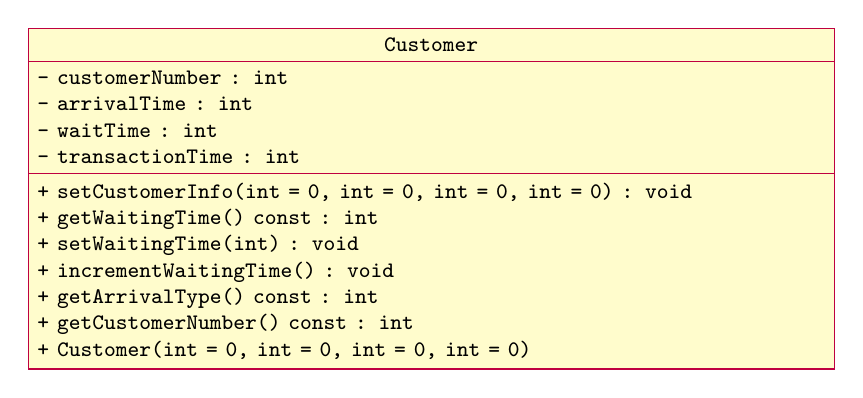
\begin{tikzpicture}[every node/.style={font=\footnotesize\ttfamily}]
    \begin{class}[text width=10cm]{Customer}{0,0}
      \attribute{- customerNumber : int}
      \attribute{- arrivalTime : int}
      \attribute{- waitTime : int}
      \attribute{- transactionTime : int}
      \operation{+ setCustomerInfo(int = 0, int = 0, int = 0, int = 0) : void}
      \operation{+ getWaitingTime() const : int}
      \operation{+ setWaitingTime(int) : void}
      \operation{+ incrementWaitingTime() : void}
      \operation{+ getArrivalType() const : int}
      \operation{+ getCustomerNumber() const : int}
      \operation{+ Customer(int = 0, int = 0, int = 0, int = 0)}
    \end{class}
  \end{tikzpicture}
\end{frame}

\begin{frame}{UML class diagram for the \texttt{Server} class}
  \center
  \renewcommand{\umlfillcolor}{CSUblue!80!black}
  \renewcommand{\umldrawcolor}{white}
  \renewcommand{\umltextcolor}{white}
  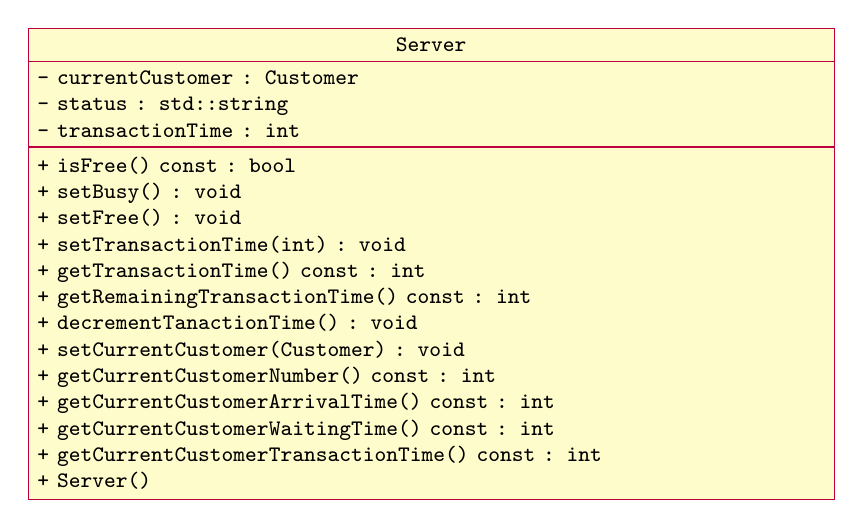
\begin{tikzpicture}[every node/.style={font=\footnotesize\ttfamily}]
    \begin{class}[text width=10cm]{Server}{0,0}
      \attribute{- currentCustomer : Customer}
      \attribute{- status : std{:}:string}
      \attribute{- transactionTime : int}
      \operation{+ isFree() const : bool}
      \operation{+ setBusy() : void}
      \operation{+ setFree() : void}
      \operation{+ setTransactionTime(int) : void}
      \operation{+ getTransactionTime() const : int}
      \operation{+ getRemainingTransactionTime() const : int}
      \operation{+ decrementTanactionTime() : void}
      \operation{+ setCurrentCustomer(Customer) : void}
      \operation{+ getCurrentCustomerNumber() const : int}
      \operation{+ getCurrentCustomerArrivalTime() const : int}
      \operation{+ getCurrentCustomerWaitingTime() const : int}
      \operation{+ getCurrentCustomerTransactionTime() const : int}
      \operation{+ Server()}
    \end{class}
  \end{tikzpicture}
\end{frame}

\begin{frame}{UML class diagram for the \texttt{ServerList} class}
  ServerList: a set of servers.\\
  At any given time, a server is either free or busy.

  \center
  \renewcommand{\umlfillcolor}{CSUblue!80!black}
  \renewcommand{\umldrawcolor}{white}
  \renewcommand{\umltextcolor}{white}
  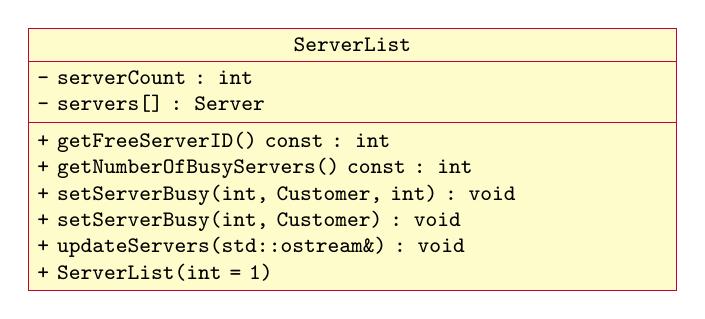
\begin{tikzpicture}[every node/.style={font=\footnotesize\ttfamily}]
    \begin{class}[text width=8cm]{ServerList}{0,0}
      \attribute{- serverCount : int}
      \attribute{- servers[] : Server}
      \operation{+ getFreeServerID() const : int}
      \operation{+ getNumberOfBusyServers() const : int}
      \operation{+ setServerBusy(int, Customer, int) : void}
      \operation{+ setServerBusy(int, Customer) : void}
      \operation{+ updateServers(std::ostream\&) : void}
      \operation{+ ServerList(int = 1)}
    \end{class}
  \end{tikzpicture}
\end{frame}

\begin{frame}{Waiting Customers Queue}
  \begin{itemize}
    \item 
      When a customer arrives, he/she goes to the end of the queue.
    \item 
      When a server becomes available, the customer at the front of the queue leaves to conduct the transaction.
    \item 
      After each time unit, the waiting time of each customer in the queue is incremented by 1.
    \item 
      Can use our Queue class but must add an operation to increment waiting time.
  \end{itemize}
\end{frame}

\begin{frame}{Algorithm for the main loop}
  For each time unit (of the clock) from 1 to the end of the simulated time:
  \begin{enumerate}
    \item 
      Updated the server list to decrement the transaction time of each busy server by one time unit.
    \item 
      If the customer's queue is nonempty, increment the waiting time of each customer by one time unit.
    \item 
      If a customer arrives, increment the customer count by 1 and add the new customer to the queue.
    \item 
      While a server is free and the customer's queue is nonempty, remove the customer from the front of the queue and send the customer to the free server.
  \end{enumerate}
\end{frame}

\section{Review}

\begin{frame}{Summary}
\begin{itemize}
\item
  \emph{Stack}: items are added/deleted from one end.
  \begin{itemize}
  \item
    Last In, First Out (LIFO) data structure
  \item
    Operations: push, pop, initialize, destroy, check for empty/full stack
  \item
    Can be implemented as an array or linked list.
  \item
    Middle elements should not be accessed directly.
  \end{itemize}
\item
  \emph{Postfix notation}: operators are written after the operands (no parentheses needed).
\end{itemize}
\end{frame}

\begin{frame}{Summary}
\begin{itemize}
\item
  \emph{Queue}: items are added at one end and removed from the other end (FIFO).
  \begin{itemize}
  \item
    First In, First Out (FIFO) data structure
  \item
    Operations: add, remove, initialize, destroy, check if the queue is empty/full
  \item
    Can be implemented as an array or linked list.
  \item
    Middle elements should not be accessed directly.
  \item
    Is a restricted version of an array or linked list.
  \end{itemize}
\end{itemize}
\end{frame}


\section*{Lab 12}
\begin{frame}{Lab 12: Stacks and Queues}
\centering\Large
  Let's take a look at Lab 12.
\end{frame}
\end{document}
